\chapter{Rate-Distortion Theory in Latent Spaces}
\label{ch:rate_distortion}

\section{The Geometry of Compression: An Introduction}

In deep learning, the representations learned by autoencoders are frequently interpreted through the lens of feature extraction, manifold learning, and dimensionality reduction. While these perspectives are powerful, they often lack a strict, quantifiable measure of representation optimality. A more fundamental perspective arises from information theory, specifically \emph{rate-distortion theory}. Formulated by Claude Shannon in 1959, rate-distortion theory establishes the absolute theoretical limits of lossy data compression. It addresses a profound question: what is the minimum number of bits per symbol (the \emph{rate}) required to represent a source signal such that it can be reconstructed with an expected error no greater than a specified threshold (the \emph{distortion})?

When applied to latent variable models such as the Variational Autoencoder (VAE), rate-distortion theory provides a rigorous mathematical framework for understanding the core trade-off governing deep generative models. It elucidates the tension between the complexity of the latent representation $z$ and the fidelity of the reconstructed input $x$. In this chapter, we explore how modern neural networks implicitly and explicitly navigate these theoretical bounds.

In an ideal, noiseless scenario, we might wish to represent our dataset $\mathcal{D} = \{x_1, \dots, x_N\} \sim P_{\text{data}}$ with zero error. However, the continuous nature of high-dimensional data—such as natural images, audio waveforms, or dense textual embeddings—implies that exact representation requires infinite precision, and thus, infinite bits. Consequently, any continuous latent space compression is inherently lossy. A neural network is forced to decide which features of the input space $\mathcal{X}$ are essential and which can be discarded as noise. This decision process is not arbitrary; it is governed by the structural constraints placed on the bottleneck.

The inference model (or encoder) $q_\phi(z|x)$ dictates the mapping from the data manifold into the latent space. The stochasticity inherent in $q_\phi(z|x)$ can be viewed mathematically as a noisy communication channel. By injecting variance into the encodings, the model limits the channel capacity, thereby constraining the rate of information flow. This is distinct from deterministic autoencoders, which must rely on explicitly restricting the dimensionality of the bottleneck. In stochastic models, even a high-dimensional latent space can have a low effective rate if the variance of the injected noise is sufficiently large relative to the signal.

The generative model (or decoder) $p_\theta(x|z)$ subsequently attempts to invert this mapping, transforming the compressed latent code back into the original data space. The quality of this inversion is measured by a distortion function, commonly the mean squared error for continuous variables or cross-entropy for categorical data. The optimization landscape is therefore a tug-of-war: the encoder is pressured to transmit more information to lower the distortion, while the prior exerts a regularizing force that penalizes high transmission rates.

By interpreting the objective functions of deep generative models through this theoretical lens, we uncover a direct correspondence between empirical optimization and the foundational limits of information theory. As we will demonstrate mathematically, the regularization terms in models like the $\beta$-VAE restrict the transmission rate, while the reconstruction terms penalize distortion. This perspective unifies disparate empirical observations and provides a principled mechanism for controlling the trade-off between latent disentanglement, aggressive compression, and generation quality.

\section{Formalizing the Rate-Distortion Trade-off}

To formalize these concepts, we consider an input space $\mathcal{X}$ populated by a random variable $X \sim P_{\text{data}}(x)$, and a latent space defined by a random variable $Z$. We further define a non-negative distortion measure $d: \mathcal{X} \times \mathcal{X} \to \mathbb{R}_{\ge 0}$, where $d(x, \hat{x})$ quantifies the cost of representing the original data point $x$ by its reconstruction $\hat{x}$.

\begin{definition}[Rate-Distortion Function]
Given a source distribution $P_{\text{data}}(x)$ and a distortion measure $d(x, \hat{x})$, the rate-distortion function $R(D)$ is defined as the minimum mutual information between $X$ and its reconstruction $\hat{X}$ such that the expected distortion is bounded by a threshold $D$:
\begin{equation}
    R(D) = \min_{p(\hat{x}|x) : \mathbb{E}[d(X, \hat{X})] \le D} I(X; \hat{X})
\end{equation}
\end{definition}

In the context of latent variable models parameterized by neural networks, the information bottleneck lies between $X$ and $Z$. The representation $Z$ is then decoded into the reconstruction $\hat{X}$. The sequence of transformations $X \to Z \to \hat{X}$ forms a Markov chain.

\begin{lemma}[Data Processing Inequality for Autoencoders]
For the Markov chain $X \to Z \to \hat{X}$ defined by an encoder $q_\phi(z|x)$ and a decoder $p_\theta(x|z)$, the mutual information satisfies:
\begin{equation}
    I(X; \hat{X}) \le I(X; Z)
\end{equation}
\end{lemma}
\begin{proof}
By the chain rule for mutual information, we can expand the joint mutual information $I(X; Z, \hat{X})$ in two equivalent ways:
\begin{align*}
    I(X; Z, \hat{X}) &= I(X; Z) + I(X; \hat{X} | Z) \\
    &= I(X; \hat{X}) + I(X; Z | \hat{X})
\end{align*}
Because $X \to Z \to \hat{X}$ is a Markov chain, $X$ and $\hat{X}$ are conditionally independent given $Z$. Therefore, $I(X; \hat{X} | Z) = 0$. This simplifies our equation to:
\begin{equation*}
    I(X; Z) = I(X; \hat{X}) + I(X; Z | \hat{X})
\end{equation*}
Since mutual information is fundamentally non-negative, $I(X; Z | \hat{X}) \ge 0$, and thus $I(X; \hat{X}) \le I(X; Z)$.
\end{proof}

This lemma has a profound implication: minimizing the rate of the latent bottleneck $I(X;Z)$ effectively places an upper bound on the true rate $I(X; \hat{X})$ transmitted through the entire autoencoder pipeline. 

\begin{figure}[htbp]
\centering
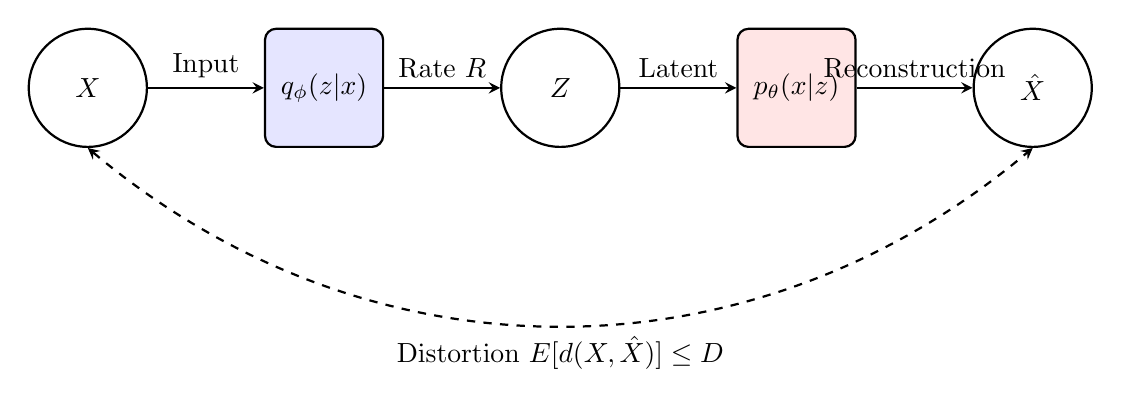
\begin{tikzpicture}[node distance=3cm, >=stealth, thick]
    % Nodes
    \node[draw, circle, minimum size=1.5cm] (X) at (0, 0) {$X$};
    \node[draw, rectangle, rounded corners, minimum size=1.5cm, fill=blue!10] (Enc) at (3, 0) {$q_\phi(z|x)$};
    \node[draw, circle, minimum size=1.5cm] (Z) at (6, 0) {$Z$};
    \node[draw, rectangle, rounded corners, minimum size=1.5cm, fill=red!10] (Dec) at (9, 0) {$p_\theta(x|z)$};
    \node[draw, circle, minimum size=1.5cm] (Xhat) at (12, 0) {$\hat{X}$};
    
    % Edges
    \draw[->] (X) -- (Enc) node[midway, above] {Input};
    \draw[->] (Enc) -- (Z) node[midway, above] {Rate $R$};
    \draw[->] (Z) -- (Dec) node[midway, above] {Latent};
    \draw[->] (Dec) -- (Xhat) node[midway, above] {Reconstruction};
    
    % Distortion annotation
    \draw[<->, dashed, bend right=40] (X.south) to node[below] {Distortion $\mathbb{E}[d(X, \hat{X})] \le D$} (Xhat.south);
\end{tikzpicture}
\caption{The Markov chain $X \to Z \to \hat{X}$ induced by an autoencoder. Information flows through the stochastic encoder, establishing a rate limit, while the decoder attempts to minimize the expected distortion.}
\label{fig:rd_markov}
\end{figure}

\begin{theorem}[VAE Objective as a Rate-Distortion Bound]
Let $q_\phi(z|x)$ be an encoder and $p_\theta(x|z)$ be a decoder. Define the distortion measure as the expected negative log-likelihood, $d(x, z) = -\log p_\theta(x|z)$. The optimization objective of the $\beta$-VAE, denoted $\mathcal{L}(\theta, \phi; \beta)$, minimizes an upper bound on the rate for a given distortion.
\end{theorem}
\begin{proof}
Consider the mutual information between the data $X$ and the latent variable $Z$ under the joint distribution $p(x, z) = P_{\text{data}}(x)q_\phi(z|x)$. We can expand $I(X;Z)$ as follows:
\begin{align}
    I(X;Z) &= \iint P_{\text{data}}(x) q_\phi(z|x) \log \frac{q_\phi(z|x)}{q_\phi(z)} \, dz \, dx \nonumber \\
    &= \mathbb{E}_{P_{\text{data}}(x)}\left[ D_{\text{KL}}(q_\phi(z|x) \parallel q_\phi(z)) \right]
\end{align}
where $q_\phi(z) = \mathbb{E}_{P_{\text{data}}(x)}[q_\phi(z|x)]$ is the aggregated posterior distribution. 

In a standard Variational Autoencoder, we specify a simple prior $p(z)$ (usually an isotropic normal distribution). We can rewrite the logarithm by introducing $p(z)$:
\begin{align}
    \mathbb{E}_{P_{\text{data}}(x)}\left[ D_{\text{KL}}(q_\phi(z|x) \parallel p(z)) \right] &= \iint P_{\text{data}}(x) q_\phi(z|x) \log \frac{q_\phi(z|x)}{p(z)} \, dz \, dx \nonumber \\
    &= \iint P_{\text{data}}(x) q_\phi(z|x) \left( \log \frac{q_\phi(z|x)}{q_\phi(z)} + \log \frac{q_\phi(z)}{p(z)} \right) \, dz \, dx \nonumber \\
    &= I(X;Z) + D_{\text{KL}}(q_\phi(z) \parallel p(z))
\end{align}
Because the Kullback-Leibler divergence is strictly non-negative ($D_{\text{KL}}(q_\phi(z) \parallel p(z)) \ge 0$), it immediately follows that:
\begin{equation}
    I(X;Z) \le \mathbb{E}_{P_{\text{data}}(x)}\left[ D_{\text{KL}}(q_\phi(z|x) \parallel p(z)) \right]
\end{equation}
This establishes an upper bound on the rate, which we denote as $R_{UB}$. 

The expected distortion under our negative log-likelihood measure is:
\begin{equation}
    D_{\text{expected}} = \mathbb{E}_{P_{\text{data}}(x)}\left[ \mathbb{E}_{q_\phi(z|x)}[-\log p_\theta(x|z)] \right]
\end{equation}
The $\beta$-VAE loss function is precisely the unconstrained Lagrangian formulation of the rate-distortion optimization problem:
\begin{equation}
    \mathcal{L}(\theta, \phi; \beta) = D_{\text{expected}} + \beta R_{UB}
\end{equation}
Thus, minimizing $\mathcal{L}(\theta, \phi; \beta)$ implicitly minimizes an upper bound on the transmission rate while explicitly minimizing the expected distortion, mapped out over the Pareto frontier by varying the Lagrange multiplier $\beta$.
\end{proof}

\begin{figure}[htbp]
\centering
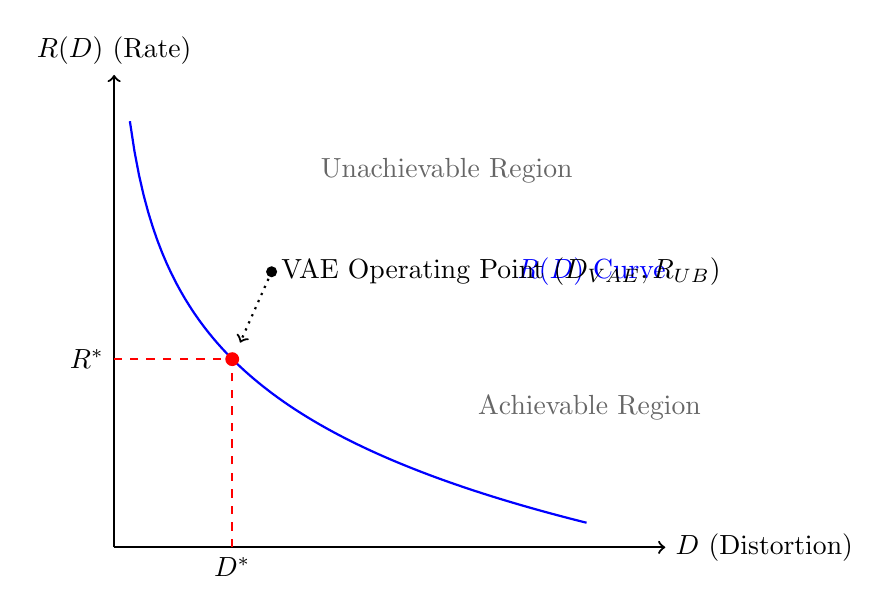
\begin{tikzpicture}
    % Axes
    \draw[->, thick] (0, 0) -- (7, 0) node[right] {$D$ (Distortion)};
    \draw[->, thick] (0, 0) -- (0, 6) node[above] {$R(D)$ (Rate)};
    
    % Curve
    \draw[thick, blue, domain=0.2:6, samples=100] plot (\x, {max(0, -1.5*ln(\x) + 3)});
    
    % Annotations
    \node at (2.5, 4.5) [anchor=south west, text=black!60] {Unachievable Region};
    \node at (4.5, 1.5) [anchor=south west, text=black!60] {Achievable Region};
    \node at (5, 3.5) [anchor=west, text=blue] {$R(D)$ Curve};
    
    % Dashed lines for a specific point
    \draw[dashed, thick, red] (1.5, 0) node[below, text=black] {$D^*$} -- (1.5, 2.39) -- (0, 2.39) node[left, text=black] {$R^*$};
    \fill[red] (1.5, 2.39) circle (2.5pt);
    
    % Example of VAE Bound
    \fill[black] (2.0, 3.5) circle (2pt) node[right] {VAE Operating Point ($D_{\text{VAE}}, R_{UB}$)};
    \draw[->, dotted, thick] (2.0, 3.5) -- (1.6, 2.6);
\end{tikzpicture}
\caption{The rate-distortion function $R(D)$ forms a monotonically decreasing, convex curve that separates achievable compressions from impossible ones. A real-world VAE operates at a point $(D_{\text{VAE}}, R_{UB})$ that is strictly sub-optimal, lying within the achievable region above the theoretical curve.}
\label{fig:rd_curve2}
\end{figure}

\subsection*{Numerical Example: The Gaussian Source}
Consider a scalar Gaussian source $X \sim \mathcal{N}(0, \sigma_x^2)$ and a squared-error distortion measure $d(x, \hat{x}) = (x - \hat{x})^2$. It is a well-known analytical result in information theory that the rate-distortion function for this continuous source is given by:
\begin{equation}
    R(D) = 
    \begin{cases} 
      \frac{1}{2} \log_2 \left( \frac{\sigma_x^2}{D} \right) & \text{if } 0 < D \le \sigma_x^2 \\
      0 & \text{if } D > \sigma_x^2
    \end{cases}
\end{equation}
Let the source variance be $\sigma_x^2 = 1$. Suppose we mandate a reconstruction with a maximum expected mean squared error of $D = 0.25$. Substituting this requirement into our formula yields the theoretical minimum transmission rate:
\begin{equation}
    R(0.25) = \frac{1}{2} \log_2\left(\frac{1}{0.25}\right) = \frac{1}{2} \log_2(4) = 1 \text{ bit}.
\end{equation}
This mathematically guarantees that any optimal encoder mapping $X$ to a continuous latent space $Z$ must transmit exactly 1 bit of mutual information per symbol to allow the decoder to achieve an MSE of 0.25. 

If a $\beta$-VAE is trained on this data, the KL divergence penalty bounds the mutual information. If this penalty term approaches 1 bit from above, the network is nearing optimal channel capacity. Conversely, if the KL term is regularized to drop below 1 bit, it is theoretically impossible for the expected reconstruction MSE to remain at or below 0.25. The generative model must allocate at least 1 bit of its latent capacity budget to encode the requisite information from $X$.

\begin{horizon}
While rate-distortion theory offers an elegant theoretical bedrock for autoencoders, closing the gap between the upper bound (the VAE objective) and the true rate-distortion function remains an active frontier. The discrepancy largely stems from the marginal KL gap $D_{\text{KL}}(q_\phi(z) \parallel p(z))$. It is conjectured that more flexible, learned priors $p_\theta(z)$—such as those parameterized by normalizing flows or diffusion processes—that dynamically adapt to the aggregated posterior $q_\phi(z)$ could virtually eliminate this gap. If achieved, neural networks could systematically operate at the true Shannon limit in high-dimensional semantic spaces.

An equally pressing open question involves the rigorous definition of distortion. Mean squared error is analytically tractable but notoriously misaligned with human perceptual judgments, especially for natural images and audio. Future work might show that mapping complex sensory data into an intermediate manifold—where simple Euclidean distance correlates perfectly with deep perceptual similarity—and subsequently applying standard rate-distortion bounds, can yield optimal generative models that simultaneously achieve maximal compression and flawless perceptual fidelity.
\end{horizon}

\section{Summary}
\begin{itemize}
    \item Rate-distortion theory defines the absolute boundaries of lossy compression, quantifying the minimum information rate $R(D)$ strictly required to achieve a target average distortion $D$.
    \item The generative $\beta$-VAE framework naturally maps onto the rate-distortion optimization problem. The KL divergence regularization term bounds the rate (mutual information), while the reconstruction loss serves as the empirical distortion measure.
    \item The theoretical gap between practical deep learning bounds and the true Shannon limit is mathematically driven by the mismatch between the aggregated posterior of the encoder and the chosen latent prior.
\end{itemize}

\section{Exercises}
\begin{enumerate}
    \item \textbf{Gaussian Rate-Distortion:} Starting from the definition of mutual information for continuous variables, derive the rate-distortion function $R(D) = \frac{1}{2}\log_2(\sigma^2 / D)$ for a zero-mean Gaussian source with variance $\sigma^2$ under squared-error distortion. Show that for $D \ge \sigma^2$, the minimum rate is identically zero.
    \item \textbf{Lagrangian Formulation:} Prove that minimizing the unconstrained Lagrangian $\mathcal{L} = D + \beta R$ traces out the convex hull of the rate-distortion curve. Explain the interpretation of the parameter $\beta$ as the negative slope of the rate-distortion function at the optimal operating point.
    \item \textbf{Tightening the VAE Bound:} Propose a mathematical modification to the standard isotropic Gaussian prior in a Variational Autoencoder that would strictly decrease the marginal KL gap $D_{\text{KL}}(q_\phi(z) \parallel p(z))$ without increasing the reconstruction distortion. Discuss the computational trade-offs of your proposed prior.
\end{enumerate}

% TODO-CITE: Ensure all named results are cited.
